
% Author: Robert McLay

\documentclass[aspectratio=169]{beamer}
\usetheme{TACC16}
\usepackage{graphicx}
\usepackage{hyperref}

\title[Lmod at EUM 26]{Lmod: The Lua-Based Environment Module System}
%\subtitle{Texas Advanced Computing Center}
\author{Robert McLay~\inst{1} \and Matthew Cawood~\inst{2} \and Taylor Ishisaka~\inst{3}}
\institute[A]{\textsuperscript{1}Texas Advanced Computing Center (Retired)\\ %
\textsuperscript{2} Dell\\ %
\textsuperscript{3} Texas Advanced Computing Center}

\date{April 22, 2026}

%% page 
%\begin{frame}{}
%  \begin{itemize}
%    \item
%  \end{itemize}
%\end{frame}
%
%% page 
%\begin{frame}[fragile]
%    \frametitle{}
% {\tiny
%    \begin{semiverbatim}
%    \end{semiverbatim}
%}
%  \begin{itemize}
%    \item
%  \end{itemize}
%
%\end{frame}
%
\begin{document}

% --- Title Slide ---
\begin{frame}
  \titlepage
\end{frame}

% --- What is Lmod ---
\begin{frame}{What is Lmod?}
  \begin{columns}
  \begin{column}{0.55\textwidth}
    \begin{itemize}
      \item Lmod is a \textbf{Lua-based environment module system} for managing software stacks on HPC systems.
      \item Supports both \textbf{Lua and Tcl modulefiles}.
      \item Enables \textbf{hierarchical MODULEPATHs}, \textbf{module families}, and \textbf{site policy enforcement}.
      \item Used at major HPC centers worldwide including TACC, NERSC,
        CSCS, and BSC.
      \item And Many Others: EasyBuild, Spack, OpenHPC
    \end{itemize}
  \end{column}
  \begin{column}{0.45\textwidth}
    \centering
    
\includegraphics[width=0.9\textwidth]{Lmod-4color@2x.png}
  \end{column}
  \end{columns}
\end{frame}

% --- Recap SC24 ---
\begin{frame}{Recap: Where We Left Off (EUM '25)}
  \begin{itemize}
    \item Focused on improving modulefile scripting, hooks, and hierarchy handling.
    \item Introduced the next-generation tracking database for usage collection.
    \item Simplified configuration and policy definition for large sites.
    \item Feedback from SC24 and EUM25 presentations drove the Lmod 9 feature roadmap.
  \end{itemize}
\end{frame}

% --- Transition Slide: From 8.x to 9.x ---
\begin{frame}{From 8.x to 9.x – What Changed Under the Hood}
  \begin{itemize}
    \item Consolidated over 60 feature and performance patches into the new 9.x branch.
    \item New dependency engine reduces redundant file reads and improves load order resolution.
    \item Tracking database re-engineered – up to \textbf{100× smaller footprint} at TACC.
    \item Expanded site-policy features: irreversible unloads, hide/forbid logic.
    \item Maintains full backward compatibility with existing 8.x
      stacks.
    \item Support for Lua 5.5 added in Lmod 9.2
  \end{itemize}
\end{frame}

% --- New Features ---
\begin{frame}{New Features and Enhancements}
  \begin{itemize}
    \item \textbf{Irreversible mode}: unloading a module can now set environment variables for cleanup.
    \item \textbf{depends\_on\_any()}: allows dependency on any member of a module set.
    \item \textbf{Enhanced hide\{\}/forbid\{\}}: expression-based
      control by user, group, or date (Stolen from Env. Modules)
    \item \textbf{Enhanced hideRegex\{\}/forbidRegex\{\}}: Hide/forbid
      with regex module names.
    \item \textbf{Optional tracking v2}: database shrinks 100× while preserving analytics.
    \item \textbf{New hooks (e.g., decorate\_module)} for module tagging and logging.
  \end{itemize}
\end{frame}

% --- Performance ---


\begin{frame}{Performance and Reliability}
  \begin{itemize}
    \item Refactored collection handling avoids NFS metadata bottlenecks.
    \item Improved \texttt{family()} logic speeds hierarchical resolution.
    \item Expanded compatibility: bash, zsh, fish, csh and nushell all supported.
    \item \textbf{nushell} support is new.
  \end{itemize}
\end{frame}

\begin{frame}{Performance (II)}
  \begin{itemize}
    \item Discussion at EasyBuild Users Meeting EUM 25 at J{\"u}lich, Germany
    \item Issues with modules with large dependencies ($>$ 50) loaded
      slowly
    \item Lmod supports \textbf{depends\_on()} and
      \textbf{depends\_on\_any()} to handle module X depends on modules
      A B C etc
    \item Lmod used to re-read all currently loaded modules to report
      any missing dependencies on module load and unload.
    \item This could be slow on disk based systems.
  \end{itemize}
\end{frame}


\begin{frame}{ModuleTable}
  \begin{itemize}
    \item Lmod stores its state in the user's environment
    \item Lmod calls this the \textbf{ModuleTable}.
    \item It is a Lua Table (what Python calls a \textbf{dict})
    \item It is base64 encoded and is stored in env. vars \textbf{\_ModuleTable001\_} etc
    \item \textbf{module --mt} to see it decoded.
  \end{itemize}
\end{frame}

% page 
\begin{frame}[fragile]
    \frametitle{Changes to ModuleTable to track dependencies}
  \begin{itemize}
    \item To remove re-reading all loaded modules
    \item Lmod now stores the dependencies in the ModuleTable 
    \item As an example module A has dependencies:
  \end{itemize}
 {\small
    \begin{semiverbatim}
\$ module --raw show A
depends_on("x/1.0")
depends_on_any("xx","yy/1.0")
    \end{semiverbatim}
}
\end{frame}

\begin{frame}[fragile]
    \frametitle{New ModuleTable}
 {\small
    \begin{semiverbatim}
_ModuleTable_ = \{
  mT = \{
    A = \{
      depT = \{
        depA = \{ \{ sn = "x", version = \{... \},\}, \},
        doaA = \{ \{
            \{ sn = "xx", version = \{...\}, \},
            \{ sn = "yy", version = \{...\}, \},
          \}, \}, \}, \},
    ...
  \},
\}
    \end{semiverbatim}
}
  \begin{itemize}
    \item where \textbf{depA} contains the list of \textbf{depend\_on} modules
    \item and \textbf{doaA} contains the list of \textbf{depend\_on\_any} modules
  \end{itemize}

\end{frame}

\begin{frame}{Performance Improvements}
  \begin{itemize}
    \item This and other changes improved module load times
      considerably
    \item Loading a module with 299 dependent modules on a Lustre
      filesystem
    \item Old: \textbf{40.2} seconds
    \item New \textbf{5.2} seconds
  \end{itemize}
\end{frame}

\begin{frame}{Performance Improvements?? not implemented}
  \begin{itemize}
    \item Lmod could maintain a ``Big'' cache with the contents of all
      modules
    \item This helps when loading a module with many dependencies (say
      5.2 to 2.2 seconds)
    \item However simple modules would also take 2.2 seconds
    \item This is not currently worth the hassle.
  \end{itemize}
\end{frame}

% --- Better Error Reporting ----
\begin{frame}{Better Error Reporting with AI agent help }
  \begin{itemize}
    \item EasyBuild Community wanted better error reporting when a
      module was not found when using the software hierarchy.
    \item Lmod's spider cache is used to build the software hierarchy.
    \item In some cases the spider cache had an error.
    \item Matthew Cawood used AI agents to find bug!
  \end{itemize}
\end{frame}

\begin{frame}
  \begin{center}
    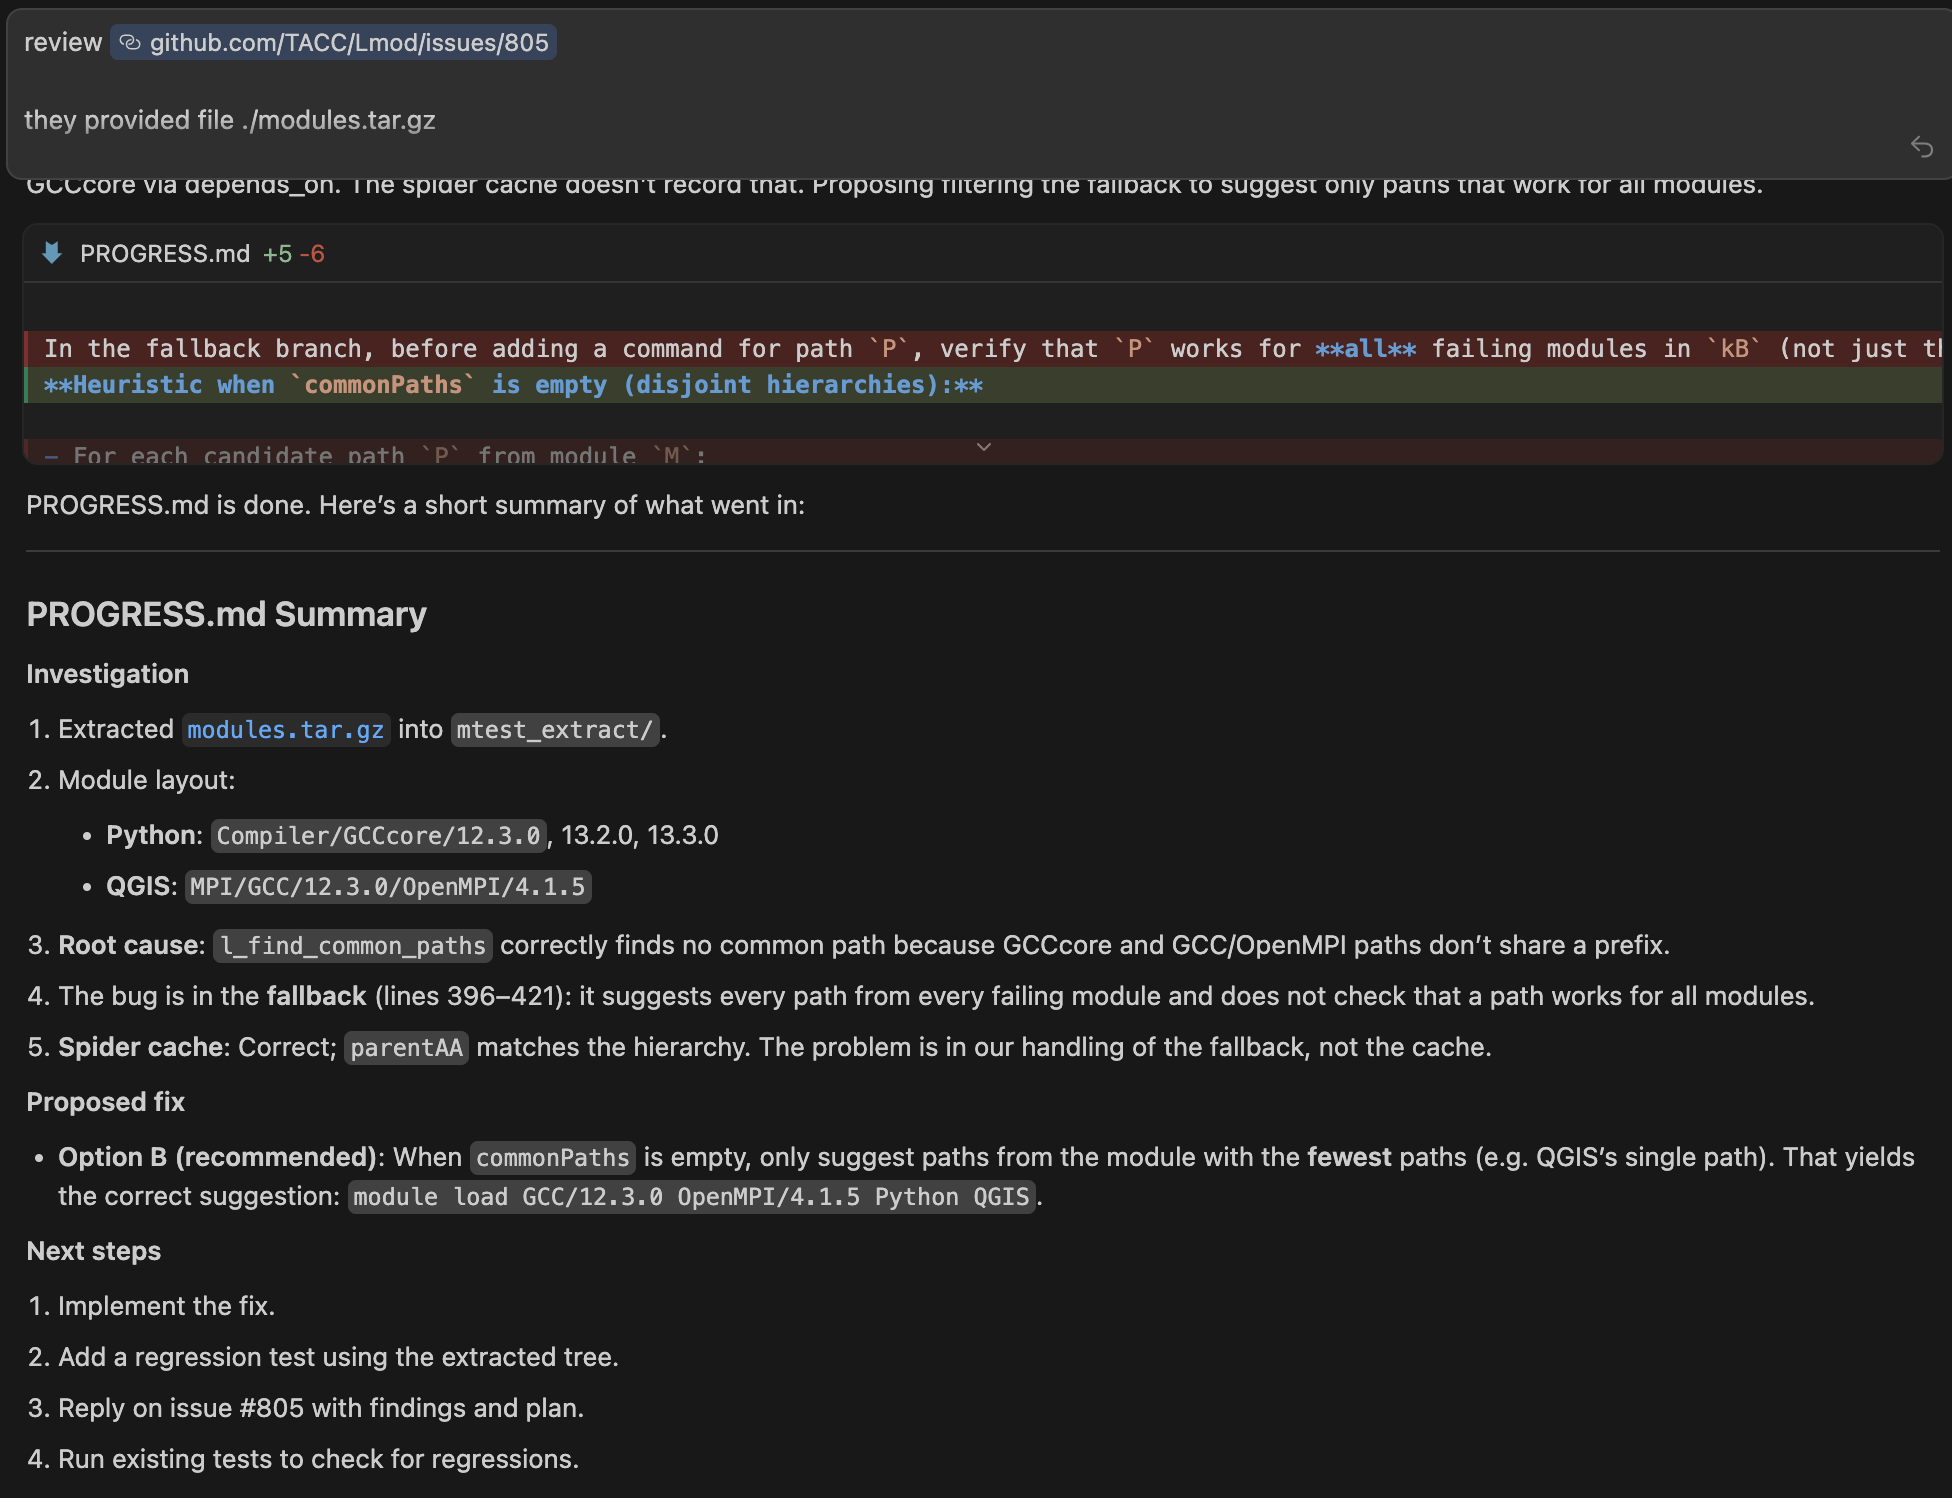
\includegraphics[width=\textwidth]{AI_805.png}
  \end{center}
\end{frame}


\begin{frame}{Upshot from AI Agents}
  \begin{itemize}
    \item Root Cause: The bug is in the fallback: lines (396-421) in src/MainControls.lua
    \item Proposed fix: When \textbf{commonPaths} is empty only suggest paths from the module with the fewest paths.
  \end{itemize}
\end{frame}

% page 
\begin{frame}[fragile]
    \frametitle{Results}
 {\small
    \begin{semiverbatim}
    $ module load Python QGIS
    Lmod has detected the following error: ...
       Try: "module spider Python QGIS" to see how to load the module(s).
       Or load any one of these options:
          module load GCC/12.3.0 OpenMPI/4.1.5 Python QGIS
    \end{semiverbatim}
}
\end{frame}

\begin{frame}{Support for Lua 5.5}
  \begin{itemize}
    \item Lua 5.5 was released late last year (2025)
    \item The major change is readonly for-loop variables
    \item Latest version of Fedora Rawhide uses Lua 5.5
    \item Lmod 9.2 supports this change
    \item Lmod depends on luaposix to do unix system functions
      (opendir etc)
    \item Luaposix is not ported to Lua 5.5 (Somehow Rawhide got
      around this)
  \end{itemize}
\end{frame}

\begin{frame}[fragile]
    \frametitle{Issue 812: Protecting Lmod from changes to LD\_LIBRARY\_PATH}
  \begin{itemize}
    \item Alan O'Cais request this change
    \item Lmod uses a way to protect LD\_LIBRARY\_PATH and LD\_PRELOAD
    \item The change is the following where the module command calls:
  \end{itemize}
 {\small
    \begin{semiverbatim}
\_\_lmod\_internal\_module\_cmd () \{
        eval "\$( \_\_LMOD\_PROTECTED\_LD\_LIBRARY\_PATH=\$LD\_LIBRARY\_PATH 
           LD\_LIBRARY\_PATH=@sys\_ld\_path@
           ...
           \$LMOD\_CMD zsh "\$@"\}"

    \end{semiverbatim}
}
\end{frame}


% --- Documentation ---
\begin{frame}{Documentation and Usability}
  \begin{itemize}
    \item Major expansion of \href{https://lmod.readthedocs.io}{lmod.readthedocs.io} with in-depth technical docs.
    \item Added sections on advanced hooks, tracking v2, and policy
      examples.
    \item Matthew Cawood used AI tools to generate much of the documentation.
    \item Clear migration guide from 8.x → 9.x.
    \item Real-world stats: TACC reduced usage DB size from 1 GB/day →
      10 MB/day.
    \item This was done by deduping data: Only one user, date, module
      per day.
    \item TACC only stores one year of data to reduce the size of the DB.
  \end{itemize}
\end{frame}

% --- Policy ---
\begin{frame}{Site Policy and Governance}
  \begin{itemize}
    \item Conditional \textbf{hide()/forbid()} rules by user, group, or time window.
    \item Deprecation warnings for outdated compilers or toolchains.
    \item Irreversible loads/unloads enable post-cleanup or variable resets.
    \item Simplifies compliance and software lifecycle management.
  \end{itemize}
\end{frame}

% --- Deployment ---
\begin{frame}{Operational Impact at TACC and Partner Sites}
  \begin{itemize}
    \item On Frontera and Stampede3: module load latency \textbf{reduced by 40\%} in deep hierarchies.
    \item Tracking database ingest reduced \textbf{100×}.
    \item GPU/CPU module tagging integrated via site hooks for usage analytics.
    \item Single \texttt{lmod\_config.lua} replaced multiple legacy init scripts.
  \end{itemize}
\end{frame}

%% --- Roadmap ----
%\begin{frame}{Looking Ahead}
%  \begin{itemize}
%    \item Ongoing performance profiling for massive module trees (>100k modules).
%    \item Additional shell and scheduler integration (Slurm, PBSPro).
%    \item Exploring distributed tracking and federated analytics.
%    \item Continued collaboration via GitHub and EUM workshops.
%  \end{itemize}
%\end{frame}

% --- Usage by Country ---
%\begin{frame}
%  \begin{center}
%    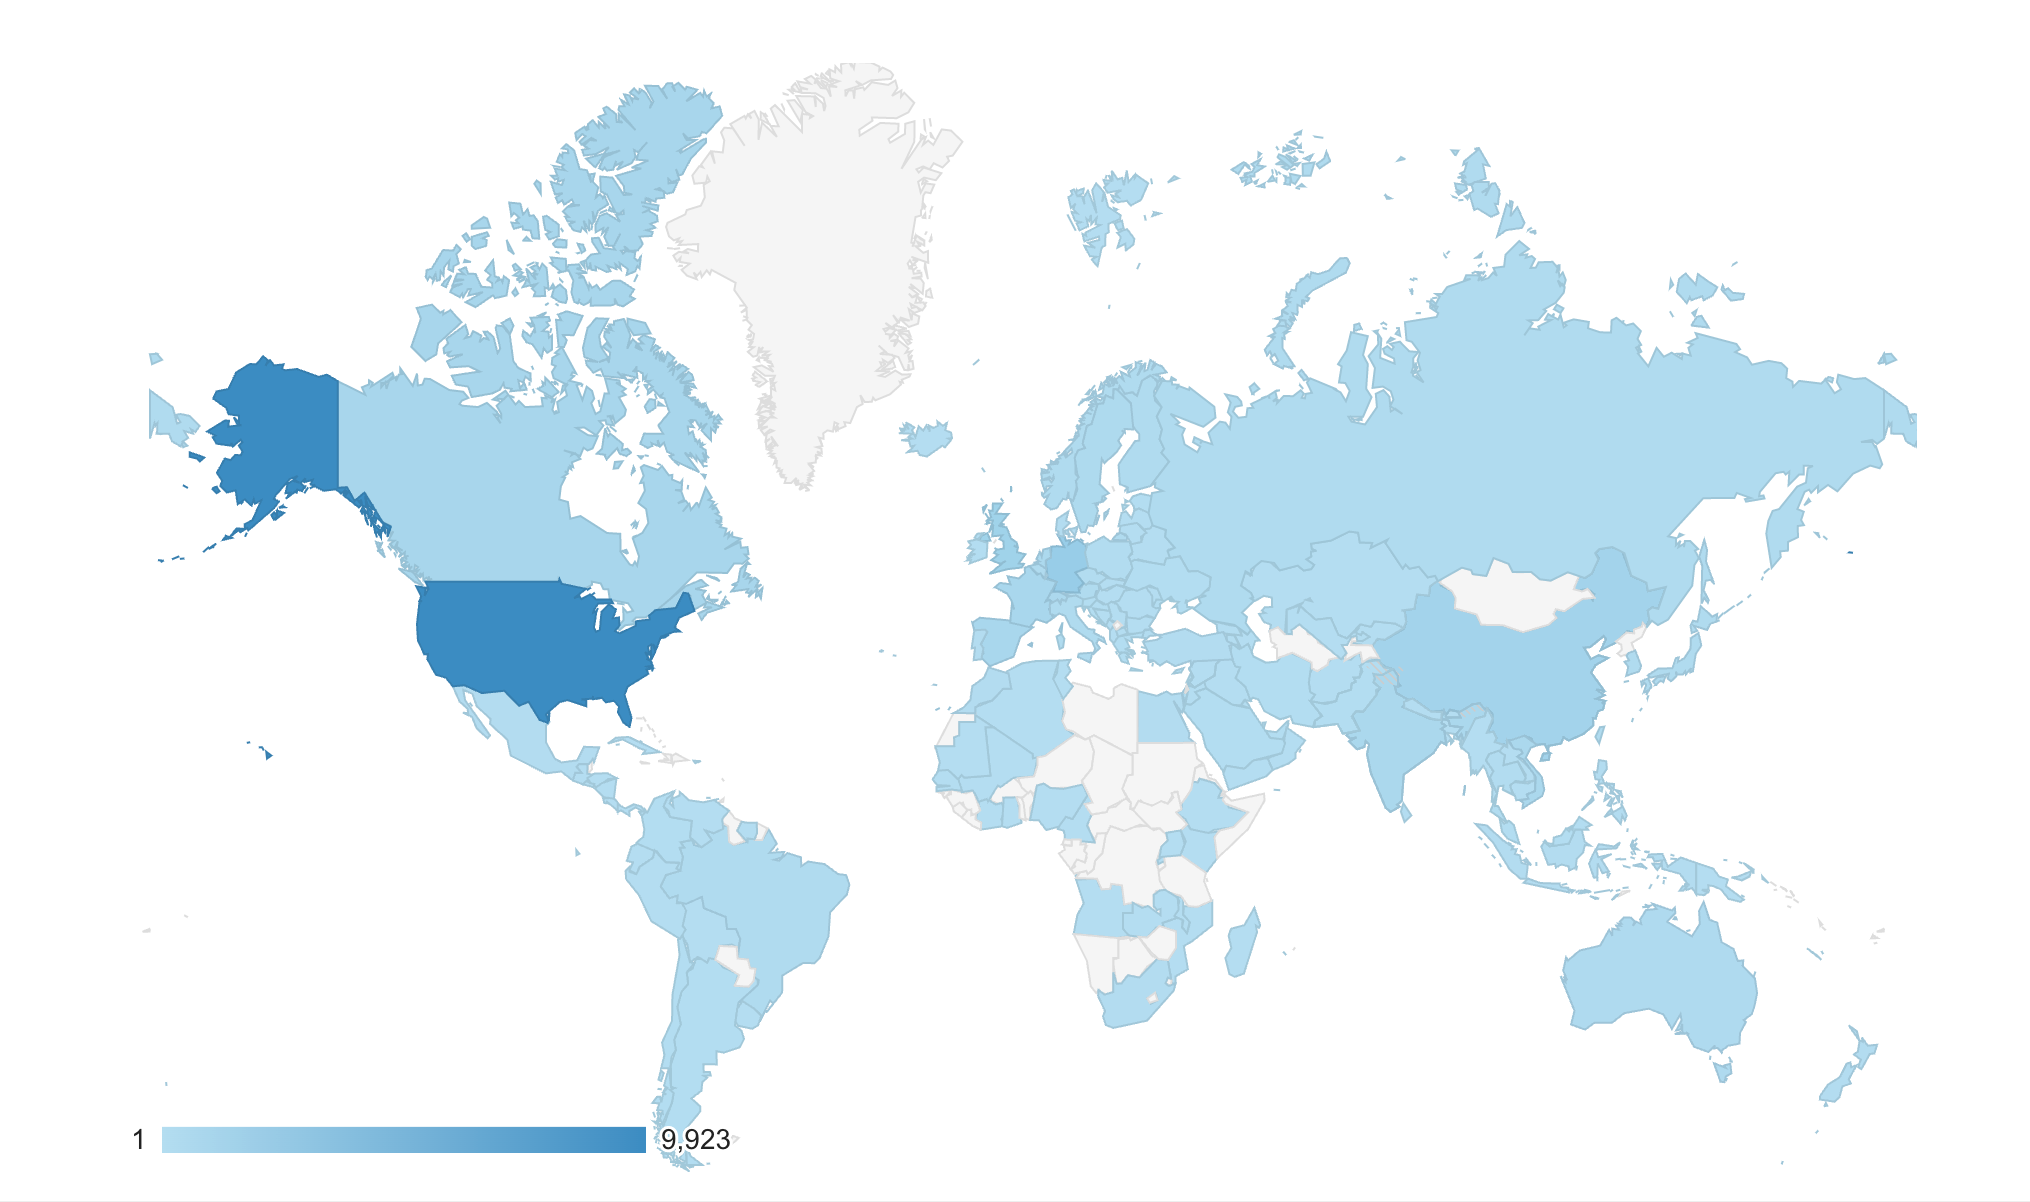
\includegraphics[width=\textwidth]{Lmod_doc_usage_by_country.png}
%  \end{center}
%\end{frame}

% --- Get Involved ---
\begin{frame}{Get Involved}
  \begin{itemize}
    \item Source: \href{https://github.com/TACC/Lmod}{github.com/TACC/Lmod}
    \item Docs: \href{https://lmod.readthedocs.io}{lmod.readthedocs.io}
    \item Mailing lists: \texttt{lmod-announce}, \texttt{lmod-users}.
    \item Contribute: report issues, propose hooks, share use cases.
    \item This Talk: https://github.com/TACC/Lmod/blob/main/my\_docs/26/EUM\_26/presentation.pdf
  \end{itemize}
\end{frame}

%% --- Final Slide ---
\begin{frame}{Thank You}
  \begin{center}
    \Large Questions? Feedback?\\[3mm]
    \Large mclay@utexas.edu\\[3mm]
    \Large Join Lmod Mailing list: https://sourceforge.net/projects/lmod/lists/lmod-users
  \end{center}
\end{frame}

\end{document}
